\documentclass{article}

% content/resources/templates/preamble.tex
\usepackage[margin=0.6in]{geometry}
\author{Milav Dabgar}
\usepackage{amsmath,amssymb,amsthm}
\usepackage{booktabs}
\usepackage{multirow}
\usepackage{xcolor}
\usepackage{tcolorbox}
\tcbuselibrary{breakable,skins}
\usepackage[colorlinks=true,linkcolor=blue]{hyperref}
\usepackage{titlesec}
\usepackage{enumitem}
\usepackage{tikz}
\usepackage{pgfplots}
\usepackage{circuitikz}
\usepackage[version=4]{mhchem}
\usepackage{longtable}
\usepackage{array}
\usepackage{float}
\usepackage{caption}
\usepackage{listings}

\lstset{
  basicstyle=\small\ttfamily,
  breaklines=true,
  breakatwhitespace=false,
  postbreak=\mbox{\textcolor{red}{$\hookrightarrow$}\space},
  float=false,
  numbers=left,
  numberstyle=\tiny\color{gray},
  numbersep=10pt,
  xleftmargin=2em,
  keywordstyle=\color{blue},
  commentstyle=\color{green!60!black},
  stringstyle=\color{purple},
  backgroundcolor=\color{gray!5},
  showstringspaces=false,
  tabsize=2,
  captionpos=b,
  keepspaces=true,
  columns=flexible
}

\pgfplotsset{compat=1.18}
\usetikzlibrary{shapes,arrows,positioning,calc,patterns,decorations.pathmorphing,decorations.markings,arrows.meta}

% Color scheme
\definecolor{headcolor}{RGB}{0,102,204}
\definecolor{keycolor}{RGB}{220,20,60}
\definecolor{solutioncolor}{RGB}{34,139,34}
\definecolor{mnemoniccolor}{RGB}{148,0,211}
\definecolor{codecolor}{RGB}{0,0,100}

% Spacing
\setlength{\parskip}{3pt}
\setlist[itemize]{nosep}
\setlist[enumerate]{nosep}

% Title formatting
\titleformat{\section}{\Large\bfseries\color{headcolor}}{\thesection}{1em}{}
\titleformat{\subsection}{\large\bfseries\color{headcolor}}{\thesubsection}{1em}{}

% Pandoc tightlist compatibility
\providecommand{\tightlist}{%
  \setlength{\itemsep}{0pt}\setlength{\parskip}{0pt}}

% Pandoc longtable compatibility
\newcounter{none}
\def\thenone{}


% content/resources/templates/english-boxes.tex

% Custom environments
\newtcolorbox{solutionbox}{
 breakable,
 enhanced,
 colback=solutioncolor!5!white,
 colframe=solutioncolor!75!black,
 fonttitle=\bfseries,
 title=Solution
}

\newtcolorbox{solutionboxnobreak}{
 colback=solutioncolor!5!white,
 colframe=solutioncolor!75!black,
 fonttitle=\bfseries,
 title=Solution
}

\newtcolorbox{keyformula}{
 breakable,
 enhanced,
 colback=keycolor!5!white,
 colframe=keycolor!75!black,
 fonttitle=\bfseries,
 title=Key Formula
}

\newtcolorbox{mnemonicboxenv}{
 breakable,
 enhanced,
 colback=mnemoniccolor!5!white,
 colframe=mnemoniccolor!75!black,
 fonttitle=\bfseries,
 title=Mnemonic
}

\newcommand{\mnemonicbox}[1]{%
  \begin{mnemonicboxenv}
    #1
  \end{mnemonicboxenv}
}


% Custom commands for GTU solutions
% This file defines semantic commands for consistent formatting

% Question command with automatic formatting
\newcommand{\question}[2]{%
  \section*{Question #1}%
  \textbf{#2}%
}

% OR question variant
\newcommand{\questionor}[2]{%
  \section*{Question #1 OR}%
  \textbf{#2}%
}

% Proper table environment with caption
\newenvironment{answertable}[1]{%
  \begin{table}[htbp]
  \centering
  \caption{#1}
}{%
  \end{table}
}

% Proper figure environment for diagrams
\newenvironment{answerdiagram}[1]{%
  \begin{figure}[htbp]
  \centering
  \caption{#1}
}{%
  \end{figure}
}

% Semantic markup for key terms
\newcommand{\keyword}[1]{\textbf{#1}}
\newcommand{\code}[1]{\texttt{#1}}
\newcommand{\classname}[1]{\texttt{#1}}
\newcommand{\methodname}[1]{\texttt{#1}}

% Proper quotation marks
\newcommand{\mnemonic}[1]{``#1''}


\title{Industrial Electronics (4331103) - Winter 2024 Solution}
\date{May 21, 2024}

\begin{document}
\maketitle

% ==========================================================================================
% Question 1
% ==========================================================================================
\questionmarks{1(a)}{3}{Draw the structure of IGBT and explain it.}

\begin{solutionbox}
IGBT combines MOSFET's input with BJT's output characteristics.

\begin{center}
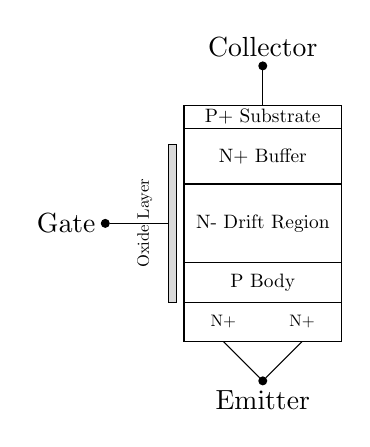
\begin{tikzpicture}[auto, node distance=2cm]
    % Terminals
    \node [draw, circle, inner sep=1pt, fill=black] (gate) at (0,2) {};
    \node [left] at (gate) {Gate};
    
    \node [draw, circle, inner sep=1pt, fill=black] (emitter) at (2,0) {};
    \node [below] at (emitter) {Emitter};
    
    \node [draw, circle, inner sep=1pt, fill=black] (collector) at (2,4) {};
    \node [above] at (collector) {Collector};
    
    % Structure
    \draw (1,0.5) rectangle (3,3.5); % Main block
    
    % Layers
    \draw (1,1) -- (3,1);
    \draw (1,1.5) -- (3,1.5);
    \draw (1,2.5) -- (3,2.5);
    \draw (1,3.2) -- (3,3.2);

    % Labels
    \node at (2, 3.35) [scale=0.7] {P+ Substrate};
    \node at (2, 2.85) [scale=0.7] {N+ Buffer};
    \node at (2, 2) [scale=0.7] {N- Drift Region};
    \node at (2, 1.25) [scale=0.7] {P Body};
    \node at (1.5, 0.75) [scale=0.6] {N+};
    \node at (2.5, 0.75) [scale=0.6] {N+};
    
    % Oxide
    \draw [fill=gray!30] (0.8, 1) rectangle (0.9, 3);
    \node at (0.5, 2) [rotate=90, scale=0.6] {Oxide Layer};
    
    % Connections
    \draw (gate) -- (0.8, 2);
    \draw (emitter) -- (1.5, 0.5);
    \draw (emitter) -- (2.5, 0.5);
    \draw (collector) -- (2, 3.5);

\end{tikzpicture}
\captionof{figure}{Structure of IGBT}
\end{center}

\begin{itemize}
    \item \keyword{Gate-Oxide Layer}: Controls device switching
    \item \keyword{N+ Emitter}: Source of electrons
    \item \keyword{P+ Collector}: Forms BJT section
\end{itemize}
\end{solutionbox}

\begin{mnemonicbox}
\mnemonic{MOSFET Input, BJT Output, IGBT Throughout}
\end{mnemonicbox}

\questionmarks{1(b)}{4}{Draw and explain the construction of SCR. Also draw the characteristic curve of it.}

\begin{solutionbox}
SCR is a four-layer PNPN semiconductor device with three terminals.

\begin{center}
\begin{tikzpicture}[auto, node distance=1.5cm]
    % Structure
    \draw (0,0) rectangle (4,2);
    \draw (1,0) -- (1,2);
    \draw (2,0) -- (2,2);
    \draw (3,0) -- (3,2);
    
    \node at (0.5,1) {P};
    \node at (1.5,1) {N};
    \node at (2.5,1) {P};
    \node at (3.5,1) {N};
    
    % Terminals
    \draw (0,1) -- (-1,1) node[left] {Anode};
    \draw (4,1) -- (5,1) node[right] {Cathode};
    \draw (2.5,0) -- (2.5,-1) node[below] {Gate};
    
    \node at (2,-1.5) {Construction};
    
    % Characteristic Curve
    \begin{scope}[xshift=7cm, yshift=-1cm]
        \draw[->] (0,2) -- (0,5) node[above] {$I_A$};
        \draw[->] (-2,2) -- (2,2) node[right] {$V_{AK}$};
        \draw[->] (0,2) -- (0,-1) node[below] {$-I_A$};
        
        % Forward Conduction
        \draw[thick, blue] (0,2) -- (1,2.2) -- (1.2, 4.5);
        \node at (1.5, 3.5) [right, scale=0.7] {Conduction};
        
        % Forward Blocking
        \draw[thick, blue, dashed] (0,2) -- (1.5, 2.2);
        \node at (1, 2.5) [scale=0.7] {Blocking};
        
        % Reverse Blocking
        \draw[thick, blue] (0,2) -- (-1.5, 2.1) -- (-1.6, 1.5);
         \node at (-1, 1.5) [left, scale=0.7] {Reverse Blocking};
        
        \node at (1.5, 2.2) [right, scale=0.7] {$V_{BO}$};
    \end{scope}
\end{tikzpicture}
\captionof{figure}{SCR Construction and V-I Characteristics}
\end{center}

\begin{itemize}
    \item \keyword{P-N-P-N Layers}: Forms two transistors (PNP, NPN)
    \item \keyword{Gate Terminal}: Triggers conduction
    \item \keyword{Holding Current}: Minimum to maintain conduction
\end{itemize}
\end{solutionbox}

\begin{mnemonicbox}
\mnemonic{PNPN Layers Form Two BJT Pairs}
\end{mnemonicbox}

\questionmarks{1(c)}{7}{Explain the working of solid state relay using Opto TRIAC, Opto-SCR and Opto-transistor with the help of circuit diagram.}

\begin{solutionbox}
Solid state relays use optocouplers for electrical isolation between control and load circuits.

\begin{center}
\begin{tikzpicture}[auto, node distance=2cm]
    % Input Side
    \node [draw, rectangle, minimum height=1cm, minimum width=2cm] (control) {Control};
    \node [right=1cm of control] (led) {};
    \draw (control) -- (led);
    \draw [->] (led) -- ++(1,0) node[midway, above] {Light};
    
    % Output Side
    \node [draw, rectangle, minimum height=3cm, minimum width=2.5cm] (iso) at (5,0) {Opto-Isolation};
    \node [right=1cm of iso] (power) {Power Switch};
    \node [right=1cm of power] (load) {Load};
    
    \draw [->] (iso) -- (power);
    \draw [->] (power) -- (load);

    % Types Box
    \node [draw, rectangle, below=1cm of iso, align=center] {Switch Types:\\TRIAC, SCR, BJT};

\end{tikzpicture}
\captionof{figure}{Solid State Relay Block Diagram}
\end{center}

\begin{center}
\captionof{table}{Types of SSR}
\begin{tabulary}{\linewidth}{|L|L|L|L|L|}
\hline
\textbf{SSR Type} & \textbf{Input Circuit} & \textbf{Isolation} & \textbf{Output Circuit} & \textbf{Applications} \\ \hline
Opto-TRIAC & DC control signal & LED + TRIAC detector & TRIAC power switch & AC loads \\ \hline
Opto-SCR & DC control signal & LED + photo-SCR & SCR power switch & DC loads \\ \hline
Opto-Transistor & DC control signal & LED + phototransistor & Power transistor & Low power DC \\ \hline
\end{tabulary}
\end{center}

\begin{itemize}
    \item \keyword{Working Principle}: Control signal activates LED $\rightarrow$ Light triggers photo-sensitive device $\rightarrow$ Switches power circuit
    \item \keyword{Zero-Crossing Detection}: Reduces EMI by switching at zero voltage
    \item \keyword{No Mechanical Parts}: Increases reliability and life
\end{itemize}
\end{solutionbox}

\begin{mnemonicbox}
\mnemonic{LED Illuminates, Photo-device Conducts, Power Flows}
\end{mnemonicbox}

\questionmarks{1(c OR)}{7}{Describe the working and constructional features of SCR, GTO and power MOSFET with the help of characteristic curve.}

\begin{solutionbox}
\begin{center}
\captionof{table}{Comparison of Devices}
\begin{tabulary}{\linewidth}{|L|L|L|L|}
\hline
\textbf{Device} & \textbf{Construction} & \textbf{Characteristic Curve} & \textbf{Working Principle} \\ \hline
SCR & PNPN 4-layer with gate & Latching - once ON stays ON & Gate pulse triggers, requires external commutation to turn OFF \\ \hline
GTO & Modified SCR with better gate control & Similar to SCR but can be turned OFF by gate & Negative gate pulse extracts carriers, turns OFF \\ \hline
Power MOSFET & Vertical structure with many cells & Non-latching - requires gate bias & Gate voltage creates channel, removed voltage turns OFF \\ \hline
\end{tabulary}
\end{center}

\begin{center}
\begin{tikzpicture}[auto, node distance=2cm]
   % SCR Symbol
   \node at (0,0) [thyristor] {};
   \node at (0,-1) {SCR};

   % GTO Symbol
   \begin{scope}[xshift=3cm]
       \node at (0,0) [gto] {};
       \node at (0,-1) {GTO};
   \end{scope}

   % MOSFET Symbol
   \begin{scope}[xshift=6cm]
       \node at (0,0) [nmos] {};
       \node at (0,-1) {MOSFET};
   \end{scope}

\end{tikzpicture}
\captionof{figure}{Device Symbols}
\end{center}

\begin{itemize}
    \item \keyword{SCR}: High current capability, latching behavior
    \item \keyword{GTO}: Self turn-off capability, higher switching speed
    \item \keyword{MOSFET}: Voltage-controlled, fast switching, no secondary breakdown
\end{itemize}
\end{solutionbox}

\begin{mnemonicbox}
\mnemonic{SCR Latches, GTO Self-Extinguishes, MOSFET Channels}
\end{mnemonicbox}

% ==========================================================================================
% Question 2
% ==========================================================================================
\questionmarks{2(a)}{3}{Explain the methods to protect SCR against over current in details.}

\begin{solutionbox}
SCR over-current protection prevents device damage due to excessive current.

\begin{center}
\captionof{table}{Over Current Protection}
\begin{tabulary}{\linewidth}{|L|L|L|}
\hline
\textbf{Protection Method} & \textbf{Working Principle} & \textbf{Implementation} \\ \hline
Fast-acting Fuses & Melts quickly during fault & Series with SCR \\ \hline
Circuit Breakers & Trips when current exceeds threshold & Main circuit protection \\ \hline
Current-limiting Reactors & Limits di/dt and peak current & Series with SCR \\ \hline
\end{tabulary}
\end{center}

\begin{itemize}
    \item \keyword{Heat Sinks}: Help dissipate excess heat
    \item \keyword{Snubber Circuits}: Reduce current spikes during switching
\end{itemize}
\end{solutionbox}

\begin{mnemonicbox}
\mnemonic{Fuses Fast, Reactors Restrict, Breakers Break}
\end{mnemonicbox}

\questionmarks{2(b)}{4}{Explain any two methods to turn ON the SCR.}

\begin{solutionbox}
SCR can be turned ON through different triggering methods.

\begin{center}
\captionof{table}{Triggering Methods}
\begin{tabulary}{\linewidth}{|L|L|L|}
\hline
\textbf{Triggering Method} & \textbf{Circuit Implementation} & \textbf{Characteristics} \\ \hline
Gate Triggering & Pulse applied between gate-cathode & Most common, controlled \\ \hline
Voltage Triggering & Anode voltage exceeds breakover voltage & No gate control, emergency \\ \hline
\end{tabulary}
\end{center}

\begin{center}
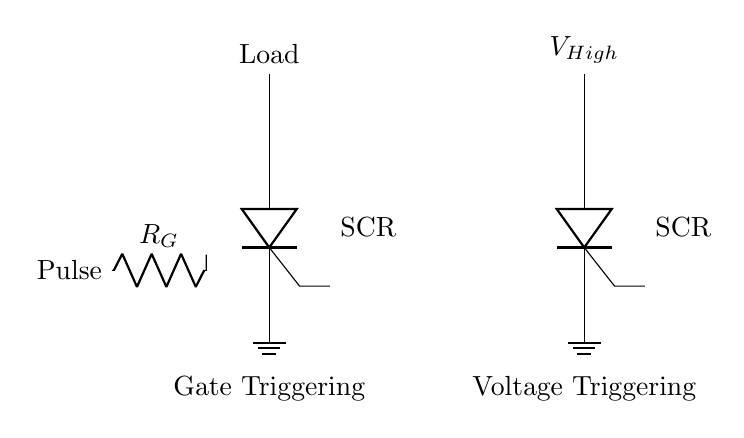
\begin{tikzpicture}[auto, node distance=2cm]
    % Gate Triggering
    \draw (0,2) node[above] {Load} -- (0,1) to[thyristor, l=SCR] (0,-1) node[ground] {};
    \draw (-2, -0.5) node[left] {Pulse} to[R, l=$R_G$] (-0.8, -0.5) -- (-0.8, -0.3); % Gate connection
    \node at (0, -2) {Gate Triggering};
    
    % Voltage Triggering
    \begin{scope}[xshift=4cm]
        \draw (0,2) node[above] {$V_{High}$} -- (0,1) to[thyristor, l=SCR] (0,-1) node[ground] {};
        \node at (0, -2) {Voltage Triggering};
    \end{scope}
\end{tikzpicture}
\captionof{figure}{SCR Turn-ON Methods}
\end{center}

\begin{itemize}
    \item \keyword{Gate Triggering}: Controls firing angle precisely
    \item \keyword{Voltage Triggering}: Happens when forward voltage exceeds breakover voltage
\end{itemize}
\end{solutionbox}

\begin{mnemonicbox}
\mnemonic{Gate Gets Control, Voltage Ventures Automatically}
\end{mnemonicbox}

\questionmarks{2(c)}{7}{Enlist the various methods to turn OFF the SCR and explain each of it using circuit diagram in brief.}

\begin{solutionbox}
SCR commutation methods are techniques to turn OFF a conducting SCR.

\begin{center}
\captionof{table}{Commutation Methods}
\begin{tabulary}{\linewidth}{|L|L|L|}
\hline
\textbf{Commutation Method} & \textbf{Circuit Principle} & \textbf{Applications} \\ \hline
Natural Commutation & AC source crosses zero & AC circuits \\ \hline
Forced Commutation & External components force current to zero & DC circuits \\ \hline
Class A (Self) & Parallel LC oscillator & Simple circuits \\ \hline
Class B (Resonant) & LC circuit in series with SCR & Medium power \\ \hline
Class C (Complementary) & Second SCR to divert current & High power \\ \hline
Class D (Auxiliary) & Auxiliary SCR + LC & Controlled timing \\ \hline
Class E (External) & External voltage source & Reliable but complex \\ \hline
\end{tabulary}
\end{center}

\begin{center}
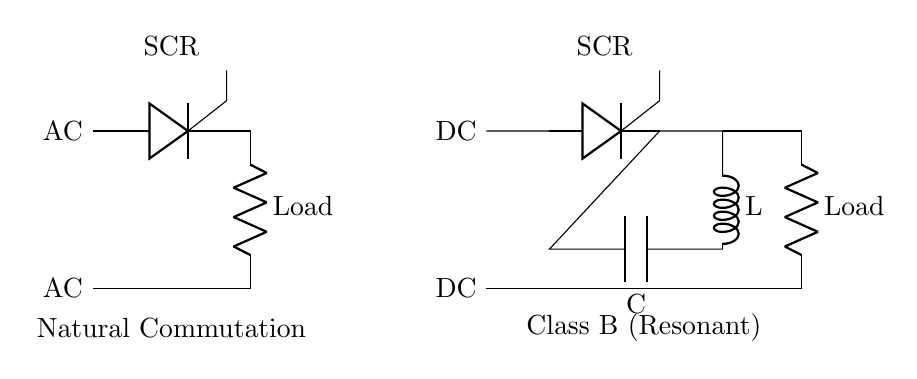
\begin{tikzpicture}[auto, node distance=1.5cm]
    % Natural Commutation
    \draw (0,0) node[left] {AC} to[thyristor, l=SCR] (2,0) to[R, l=Load] (2,-2) -- (0,-2) node[left] {AC};
    \node at (1, -2.5) {Natural Commutation};
    
    % Class B Commutation Schematic
    \begin{scope}[xshift=5cm]
         \draw (0,0) node[left] {DC} to[thyristor, l=SCR, n=scr] (3,0) -- (3,-0.5) to[L, l=L] (3,-1.5) to[C, l=C] (0.8,-1.5) -- (scr.cathode);
         \draw (3,0) -- (4,0) to[R, l=Load] (4,-2) -- (0,-2) node[left] {DC};
         \node at (2, -2.5) {Class B (Resonant)};
    \end{scope}
\end{tikzpicture}
\captionof{figure}{Commutation Circuits}
\end{center}

\begin{itemize}
    \item \keyword{Natural Commutation}: Current naturally falls to zero in AC cycles
    \item \keyword{Forced Commutation}: Artificially brings current to zero in DC circuits
    \item \keyword{Communication Classes}: A through E progressively more complex and reliable
\end{itemize}
\end{solutionbox}

\begin{mnemonicbox}
\mnemonic{Natural Zeros, Forced Components, Classes Advance Reliability}
\end{mnemonicbox}

\questionmarks{2(a OR)}{3}{Explain the methods to protect SCR against over voltage in details.}

\begin{solutionbox}
Over-voltage protection prevents damage from voltage transients.

\begin{center}
\captionof{table}{Over Voltage Protection}
\begin{tabulary}{\linewidth}{|L|L|L|}
\hline
\textbf{Protection Method} & \textbf{Working Principle} & \textbf{Implementation} \\ \hline
Snubber Circuits & RC network limits dv/dt & Parallel with SCR \\ \hline
Metal Oxide Varistors & Clamps voltage spikes & Parallel with SCR \\ \hline
Zener Diodes & Breaks down at set voltage & Anode-cathode protection \\ \hline
\end{tabulary}
\end{center}

\begin{center}
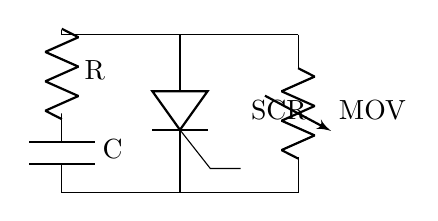
\begin{tikzpicture}[auto, node distance=2cm]
    \draw (0,2) to[thyristor, l=SCR, n=scr] (0,0);
    \draw (-1.5, 2) -- (0,2);
    \draw (-1.5, 2) to[R, l=R] (-1.5, 1) to[C, l=C] (-1.5, 0) -- (0,0);
    \draw (1.5, 2) -- (0,2);
    \draw (1.5, 2) to[vR, l=MOV] (1.5, 0) -- (0,0);
\end{tikzpicture}
\captionof{figure}{Snubber and MOV Protection}
\end{center}

\begin{itemize}
    \item \keyword{Snubber Circuit}: Limits voltage rise rate (dv/dt)
    \item \keyword{MOV}: Absorbs energy from voltage spikes
    \item \keyword{Thyristor Rating}: Always use components with margin above circuit voltage
\end{itemize}
\end{solutionbox}

\begin{mnemonicbox}
\mnemonic{Snubbers Slow, Varistors Clamp, Zeners Zap}
\end{mnemonicbox}

\questionmarks{2(b OR)}{4}{Explain triggering of Thyristor in detail.}

\begin{solutionbox}
Thyristor triggering involves activating the device from blocking to conduction state.

\begin{center}
\captionof{table}{Thyristor Triggering}
\begin{tabulary}{\linewidth}{|L|L|L|}
\hline
\textbf{Triggering Method} & \textbf{Working Mechanism} & \textbf{Advantages} \\ \hline
Gate Triggering & Low power pulse at gate-cathode & Precise control \\ \hline
R-C Phase Shift & Varies phase angle for control & Simple circuit \\ \hline
UJT Triggering & Relaxation oscillator generates pulses & Stable timing \\ \hline
Light Triggering & Photons generate carriers (LASCR) & Electrical isolation \\ \hline
\end{tabulary}
\end{center}

\begin{itemize}
    \item \keyword{Gate Current}: Must exceed latching current
    \item \keyword{Gate Pulse}: Width and amplitude critical for reliable triggering
    \item \keyword{Triggering Angle}: Controls power delivered to load
\end{itemize}
\end{solutionbox}

\begin{mnemonicbox}
\mnemonic{Gate Gets Going, RC Rhythmically, UJT Uniformly, Light Liberates}
\end{mnemonicbox}

\questionmarks{2(c OR)}{7}{Design and explain snubber circuit for SCR. Also explain the importance of it.}

\begin{solutionbox}
Snubber circuits protect SCR from voltage transients and control switching behavior.

\begin{center}
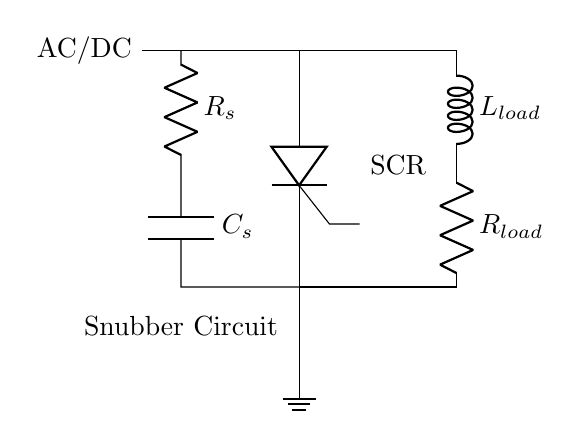
\begin{tikzpicture}[auto, node distance=2cm]
    \draw (0,4) node[left] {AC/DC} -- (2,4) -- (4,4);
    
    % SCR
    \draw (2,4) to[thyristor, l=SCR] (2,1);
    
    % Snubber
    \draw (0.5, 4) to[R, l=$R_s$] (0.5, 2.5) to[C, l=$C_s$] (0.5, 1) -- (2,1);
    
    % Load
    \draw (4,4) to[L, l=$L_{load}$] (4,2.5) to[R, l=$R_{load}$] (4,1) -- (2,1) -- (2,0) node[ground] {};
    
    \node at (0.5, 0.5) {Snubber Circuit};
\end{tikzpicture}
\captionof{figure}{SCR with Snubber Circuit}
\end{center}

\begin{center}
\captionof{table}{Snubber Components}
\begin{tabulary}{\linewidth}{|L|L|L|}
\hline
\textbf{Component} & \textbf{Function} & \textbf{Selection Criteria} \\ \hline
Resistor (R) & Limits discharge current & $R > E/I_{max}$ \\ \hline
Capacitor (C) & Absorbs voltage transients & $C = I_{load}/(dv/dt)$ \\ \hline
Optional Diode & Provides discharge path & Fast recovery type \\ \hline
\end{tabulary}
\end{center}

\textbf{Design Steps:}
\begin{enumerate}
    \item Calculate maximum dv/dt from SCR datasheet
    \item Determine load current and circuit voltage
    \item Select C to limit dv/dt below SCR rating
    \item Select R to limit discharge current and provide damping
\end{enumerate}

\textbf{Importance:}
\begin{itemize}
    \item \keyword{dv/dt Protection}: Prevents false triggering
    \item \keyword{Turn-off Support}: Improves commutation
    \item \keyword{Switching Loss Reduction}: Reduces power dissipation
    \item \keyword{EMI Reduction}: Smooths voltage transitions
\end{itemize}
\end{solutionbox}

\begin{mnemonicbox}
\mnemonic{Resistor Restrains, Capacitor Catches, Diode Directs}
\end{mnemonicbox}

% ==========================================================================================
% Question 3
% ==========================================================================================
\questionmarks{3(a)}{3}{Explain the working of three phase Full Wave Rectifier using circuit diagram.}

\begin{solutionbox}
Three-phase full-wave rectifier converts three-phase AC to DC with six diodes.

\begin{center}
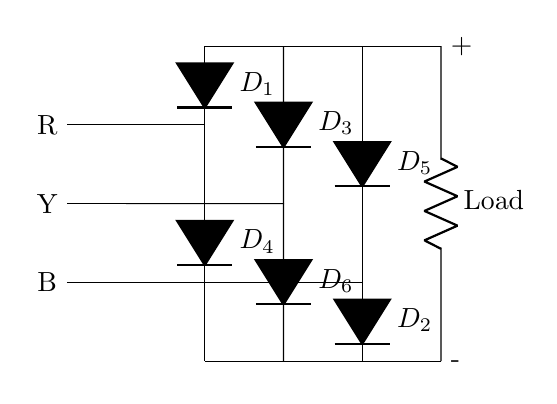
\begin{tikzpicture}[auto, node distance=1.5cm]
    % AC Source
    \node (A) at (0,3) {R};
    \node (B) at (0,2) {Y};
    \node (C) at (0,1) {B};
    
    % Bridge
    \draw (A) -- (1,3);
    \draw (B) -- (1,2);
    \draw (C) -- (1,1);
    
    % Leg 1
    \draw (2,4) to[D*, l=$D_1$] (2,3) -- (1,3);
    \draw (2,3) to[D*, l=$D_4$] (2,0);
    
    % Leg 2
    \draw (3,4) to[D*, l=$D_3$] (3,2) -- (1,2);
    \draw (3,2) to[D*, l=$D_6$] (3,0);
    
    % Leg 3
    \draw (4,4) to[D*, l=$D_5$] (4,1) -- (1,1);
    \draw (4,1) to[D*, l=$D_2$] (4,0);
    
    % Rails
    \draw (2,4) -- (5,4) node[right] {+};
    \draw (2,0) -- (5,0) node[right] {-};
    
    % Load
    \draw (5,4) to[R, l=Load] (5,0);
    
\end{tikzpicture}
\captionof{figure}{Three Phase Bridge Rectifier}
\end{center}

\begin{itemize}
    \item \keyword{Six Diodes}: Three for positive, three for negative half-cycles
    \item \keyword{Conduction}: Each diode conducts for 120\textdegree{} per cycle
    \item \keyword{Output}: Low ripple (4.2\%) compared to single-phase
\end{itemize}
\end{solutionbox}

\begin{mnemonicbox}
\mnemonic{Six Diodes, Three Phases, Smooth DC}
\end{mnemonicbox}

\questionmarks{3(b)}{4}{Differentiate single phase and poly phase rectifier circuit.}

\begin{solutionbox}
\begin{center}
\captionof{table}{Comparison of Rectifiers}
\begin{tabulary}{\linewidth}{|L|L|L|}
\hline
\textbf{Parameter} & \textbf{Single Phase Rectifier} & \textbf{Poly Phase Rectifier} \\ \hline
Input & Single AC source & Multiple AC sources (3 or more) \\ \hline
Diodes Required & 2 (half-wave), 4 (full-wave) & 3 (half-wave), 6 (full-wave) \\ \hline
Ripple Factor & 0.482 (full-wave) & 0.042 (3-phase full-wave) \\ \hline
Transformer Utilization & Lower (0.812) & Higher (0.955) \\ \hline
Output Waveform & Pulsating & Much smoother \\ \hline
Efficiency & Lower & Higher \\ \hline
Applications & Low power applications & Industrial power supplies \\ \hline
\end{tabulary}
\end{center}

\begin{itemize}
    \item \keyword{Form Factor}: Lower in poly-phase (better quality DC)
    \item \keyword{Power Handling}: Polyphase handles higher power more efficiently
    \item \keyword{Circuit Complexity}: Polyphase more complex but better performance
\end{itemize}
\end{solutionbox}

\begin{mnemonicbox}
\mnemonic{Single Pulses Heavily, Poly Provides Smoothly}
\end{mnemonicbox}

\questionmarks{3(c)}{7}{Describe the application of series, parallel and bridge type Inverter.}

\begin{solutionbox}
\begin{center}
\captionof{table}{Inverter Types}
\begin{tabulary}{\linewidth}{|L|L|L|L|}
\hline
\textbf{Inverter Type} & \textbf{Circuit Topology} & \textbf{Applications} & \textbf{Characteristics} \\ \hline
Series Inverter & Resonant LC with load in series & Induction heating, Ultrasonic generators & • High frequency \newline • Voltage source \newline • Self-commutating \\ \hline
Parallel Inverter & Resonant LC with load in parallel & Uninterruptible power supplies, Solar inverters & • Current source \newline • Better efficiency \newline • Wider load range \\ \hline
Bridge Inverter & H-bridge with 4 switches & Motor drives, Grid-tied systems, General purpose & • Voltage/current source \newline • Most versatile \newline • Various control methods \\ \hline
\end{tabulary}
\end{center}

\begin{center}
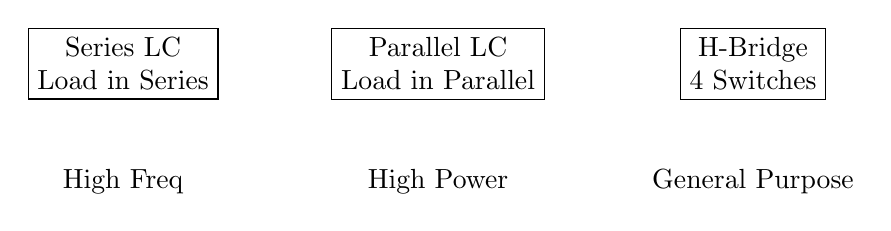
\begin{tikzpicture}[auto, node distance=1.5cm]
    % Series
    \node[draw, align=center] (series) at (0,0) {Series LC\\Load in Series};
    
    % Parallel
    \node[draw, align=center] (parallel) at (4,0) {Parallel LC\\Load in Parallel};
    
    % Bridge
    \node[draw, align=center] (bridge) at (8,0) {H-Bridge\\4 Switches};
    
    \node at (0,-1.5) {High Freq};
    \node at (4,-1.5) {High Power};
    \node at (8,-1.5) {General Purpose};
\end{tikzpicture}
\captionof{figure}{Inverter Topologies}
\end{center}

\begin{itemize}
    \item \keyword{Series Inverter}: Best for fixed-frequency, fixed-load applications
    \item \keyword{Parallel Inverter}: Handles load variations better
    \item \keyword{Bridge Inverter}: Most widely used for general applications
\end{itemize}
\end{solutionbox}

\begin{mnemonicbox}
\mnemonic{Series Sings at High Frequency, Parallel Performs with Variety, Bridge Brings Versatility}
\end{mnemonicbox}

% ==========================================================================================
% Question 3 (OR)
% ==========================================================================================

\questionmarks{3(a OR)}{3}{Explain the working of three phase Half Wave Rectifier using circuit diagram.}

\begin{solutionbox}
Three-phase half-wave rectifier uses three diodes to convert three-phase AC to DC.

\begin{center}
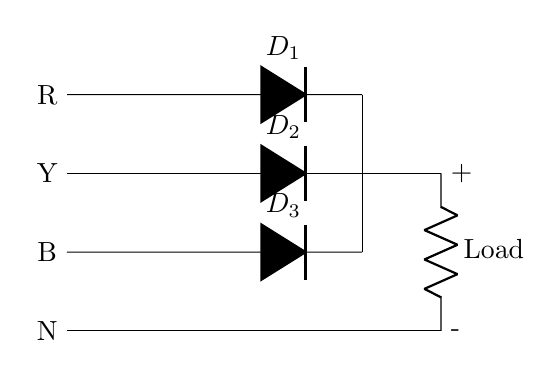
\begin{tikzpicture}[auto, node distance=1.5cm]
    % AC Source
    \node (A) at (0,3) {R};
    \node (B) at (0,2) {Y};
    \node (C) at (0,1) {B};
    \node (N) at (0,0) {N};
    
    % Diodes
    \draw (A) -- (2,3) to[D*, l=$D_1$] (4,3);
    \draw (B) -- (2,2) to[D*, l=$D_2$] (4,2);
    \draw (C) -- (2,1) to[D*, l=$D_3$] (4,1);
    
    % Output
    \draw (4,3) -- (4,1); % Common Cathode
    \draw (4,2) -- (5,2) node[right] {+};
    
    % Neutral
    \draw (N) -- (5,0) node[right] {-};
    
    % Load
    \draw (5,2) to[R, l=Load] (5,0);
    
\end{tikzpicture}
\captionof{figure}{Three Phase Half Wave Rectifier}
\end{center}

\begin{itemize}
    \item \keyword{Three Diodes}: Each conducts during positive half-cycle of its phase
    \item \keyword{Conduction}: Each diode conducts for 120\textdegree{} per cycle
    \item \keyword{Output}: 13.4\% ripple (higher than full-wave)
\end{itemize}
\end{solutionbox}

\begin{mnemonicbox}
\mnemonic{Three Diodes, Three Phases, One Direction}
\end{mnemonicbox}

\questionmarks{3(b OR)}{4}{Enlist the different types of charging technology and compare it.}

\begin{solutionbox}
\begin{center}
\captionof{table}{Charging Technologies}
\begin{tabulary}{\linewidth}{|L|L|L|L|}
\hline
\textbf{Charging Technology} & \textbf{Working Principle} & \textbf{Advantages} & \textbf{Disadvantages} \\ \hline
Constant Current (CC) & Fixed current until voltage threshold & Simple, low cost & Longer charging time \\ \hline
Constant Voltage (CV) & Fixed voltage with declining current & Fast initial charge & Current not limited at start \\ \hline
CC-CV & Starts with CC, switches to CV & Optimal charging profile & Requires controller circuit \\ \hline
Pulse Charging & Current pulses with rest periods & Reduces heat, extends battery life & Complex control circuit \\ \hline
Trickle Charging & Very low constant current & Maintains charge & Not suitable for main charging \\ \hline
Fast Charging & High current with intelligent control & Significantly reduced charging time & Heat generation, battery stress \\ \hline
Wireless Charging & Inductive coupling & Convenient, no cables & Lower efficiency, alignment issues \\ \hline
\end{tabulary}
\end{center}

\begin{itemize}
    \item \keyword{Battery Types}: Different technologies suit different battery chemistries
    \item \keyword{Charging Profiles}: Must match battery specifications to avoid damage
    \item \keyword{Temperature Management}: Critical factor in charging efficiency and safety
\end{itemize}
\end{solutionbox}

\begin{mnemonicbox}
\mnemonic{Current Consistently, Voltage Varies, Pulse Pauses, Trickle Tops, Fast Finishes}
\end{mnemonicbox}

\questionmarks{3(c OR)}{7}{Explain the working of Solar Photovoltaic (PV) based power generation with the help of block diagram.}

\begin{solutionbox}
Solar PV systems convert sunlight directly into electricity through the photovoltaic effect.

\begin{center}
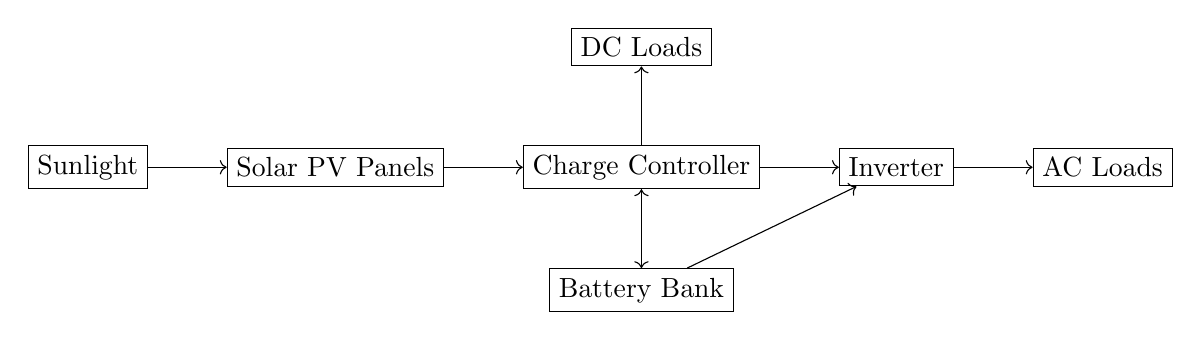
\begin{tikzpicture}[auto, node distance=2cm]
    \node [draw, rectangle] (sun) {Sunlight};
    \node [draw, rectangle, right=1cm of sun] (pv) {Solar PV Panels};
    \node [draw, rectangle, right=1cm of pv] (cc) {Charge Controller};
    \node [draw, rectangle, below=1cm of cc] (batt) {Battery Bank};
    \node [draw, rectangle, right=1cm of cc] (inv) {Inverter};
    \node [draw, rectangle, right=1cm of inv] (ac) {AC Loads};
    \node [draw, rectangle, above=1cm of cc] (dc) {DC Loads};
    
    \draw [->] (sun) -- (pv);
    \draw [->] (pv) -- (cc);
    \draw [->] (cc) -- (batt);
    \draw [->] (batt) -- (cc); % Bidirectional typically
    \draw [->] (cc) -- (inv);
    \draw [->] (inv) -- (ac);
    \draw [->] (cc) -- (dc);
    \draw [->] (batt) -- (inv); % Direct battery to inverter often

\end{tikzpicture}
\captionof{figure}{Solar PV System}
\end{center}

\begin{center}
\captionof{table}{PV System Components}
\begin{tabulary}{\linewidth}{|L|L|L|}
\hline
\textbf{Component} & \textbf{Function} & \textbf{Types} \\ \hline
Solar Panels & Convert light to DC electricity & Monocrystalline, Polycrystalline, Thin-film \\ \hline
Charge Controller & Regulates battery charging & PWM, MPPT \\ \hline
Battery Bank & Stores energy & Lead-acid, Lithium-ion, Flow \\ \hline
Inverter & Converts DC to AC & Pure sine wave, Modified sine wave \\ \hline
Distribution System & Delivers power to loads & Off-grid, Grid-tied, Hybrid \\ \hline
\end{tabulary}
\end{center}

\begin{itemize}
    \item \keyword{Photovoltaic Effect}: Light energy creates electron flow in semiconductor material
    \item \keyword{Maximum Power Point Tracking}: Optimizes power extraction under varying conditions
    \item \keyword{Grid Integration}: Can operate standalone or connected to utility grid
\end{itemize}
\end{solutionbox}

\begin{mnemonicbox}
\mnemonic{Sunlight Strikes Semiconductors, Controllers Charge, Batteries Bank, Inverters Interface}
\end{mnemonicbox}

% ==========================================================================================
% Question 4
% ==========================================================================================
\questionmarks{4(a)}{3}{State the merits and demerits of Induction heating.}

\begin{solutionbox}
\begin{center}
\captionof{table}{Induction Heating Pros and Cons}
\begin{tabulary}{\linewidth}{|L|L|}
\hline
\textbf{Merits of Induction Heating} & \textbf{Demerits of Induction Heating} \\ \hline
Rapid heating without direct contact & High initial installation cost \\ \hline
Precise temperature control & Requires electrical power source \\ \hline
Energy efficient (80-90\%) & Limited to electrically conductive materials \\ \hline
Clean and pollution-free & Requires proper cooling systems \\ \hline
Localized heating possible & EMI generation may affect nearby electronics \\ \hline
Uniform heating throughout material & May require specialized coil designs \\ \hline
\end{tabulary}
\end{center}

\begin{itemize}
    \item \keyword{Working Principle}: Eddy currents induced in workpiece generate heat
    \item \keyword{Applications}: Melting, hardening, annealing, welding
\end{itemize}
\end{solutionbox}

\begin{mnemonicbox}
\mnemonic{Fast, Focused, Efficient but Costly, Conductive, Complex}
\end{mnemonicbox}

\questionmarks{4(b)}{4}{Draw the circuit of sequential timer using IC-555 and explain its working.}

\begin{solutionbox}
Sequential timer provides multiple timed outputs in sequence.

\begin{center}
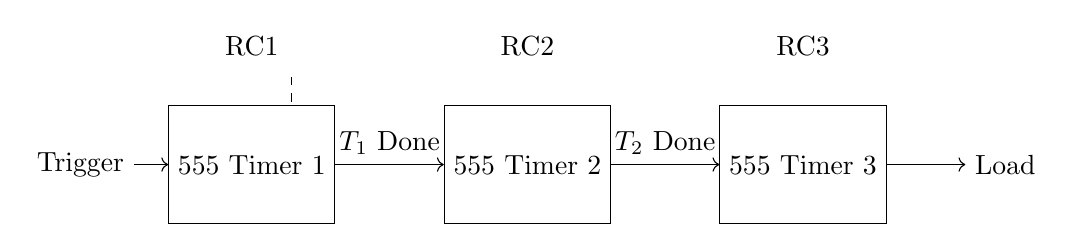
\begin{tikzpicture}[auto, node distance=2.5cm]
    % IC Blocks
    \node [draw, rectangle, minimum height=1.5cm, minimum width=2cm] (IC1) {555 Timer 1};
    \node [draw, rectangle, minimum height=1.5cm, minimum width=2cm, right of=IC1, node distance=3.5cm] (IC2) {555 Timer 2};
    \node [draw, rectangle, minimum height=1.5cm, minimum width=2cm, right of=IC2, node distance=3.5cm] (IC3) {555 Timer 3};
    
    % Connections
    \draw [->] (-1.5, 0) node[left] {Trigger} -- (IC1.west);
    \draw [->] (IC1.east) -- (IC2.west) node[midway, above] {$T_1$ Done};
    \draw [->] (IC2.east) -- (IC3.west) node[midway, above] {$T_2$ Done};
    \draw [->] (IC3.east) -- ++(1,0) node[right] {Load};
    
    % RC components abstract
    \node [above=0.5cm of IC1] {RC1};
    \node [above=0.5cm of IC2] {RC2};
    \node [above=0.5cm of IC3] {RC3};
    
    \draw [dashed] (0.5, 0.8) -- (0.5, 1.2);
    
\end{tikzpicture}
\captionof{figure}{Sequential Timer Block Diagram}
\end{center}

\textbf{Working:}
\begin{enumerate}
    \item First 555 timer operates in monostable mode
    \item Output triggers second timer when first timing cycle completes
    \item Second timer triggers third timer
    \item Each timer's period determined by its RC time constant
\end{enumerate}

\begin{itemize}
    \item \keyword{RC Values}: T = 1.1 $\times$ R $\times$ C determines each stage's timing
    \item \keyword{Cascading}: Multiple stages provide sequential timing events
    \item \keyword{Applications}: Process control, industrial sequencing
\end{itemize}
\end{solutionbox}

\begin{mnemonicbox}
\mnemonic{One Timer Triggers Another Sequentially}
\end{mnemonicbox}

\questionmarks{4(c)}{7}{Draw the schematic circuit for single phase AC power control using TRIAC and explain it in detail.}

\begin{solutionbox}
TRIAC-based AC power control regulates power to loads through phase angle control.

\begin{center}
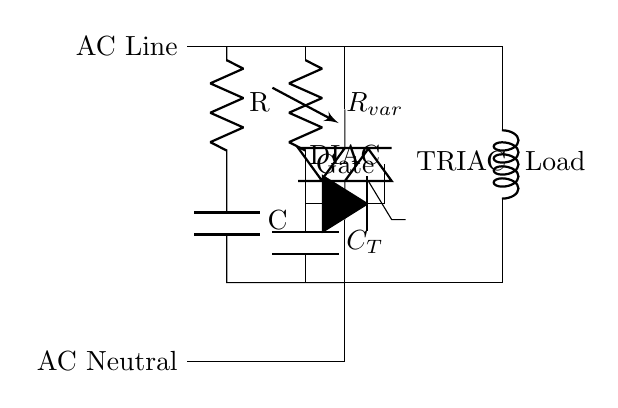
\begin{tikzpicture}[auto, node distance=2cm]
    % Power Circuit
    \draw (0,4) node[left] {AC Line} -- (2,4) -- (4,4);
    \draw (2,4) to[triac, l=TRIAC] (2,1); % Using triac component
    \draw (4,4) to[L, l=Load] (4,1) -- (2,1) -- (2,0) -- (0,0) node[left] {AC Neutral};
    
    % Control Circuit
    \draw (0.5, 4) to[R, l=R] (0.5, 2.5) to[C, l=C] (0.5, 1) -- (2,1); % Snubber
    
    % Triggering
    \draw (1.5, 4) to[vR, l=$R_{var}$] (1.5, 2.5) -- (1.5, 2);
    \draw (1.5, 2) to[C, l=$C_T$] (1.5, 1);
    \draw (1.5, 2) to[D*, l=DIAC] (2.5, 2) -- (2.5, 2.5); % Connect to Gate
    \node at (2.5, 2.5) [left] {Gate};
    
\end{tikzpicture}
\captionof{figure}{TRIAC Power Control Circuit}
\end{center}

\begin{center}
\captionof{table}{Circuit Components}
\begin{tabulary}{\linewidth}{|L|L|L|}
\hline
\textbf{Component} & \textbf{Function} & \textbf{Selection Criteria} \\ \hline
TRIAC & Bidirectional power switch & Current rating > load current \\ \hline
DIAC & Triggers TRIAC symmetrically & Breakover voltage < trigger voltage \\ \hline
RC Network & Phase shifting for firing angle & R determines firing angle range \\ \hline
Snubber Circuit & dv/dt protection & Based on TRIAC specifications \\ \hline
\end{tabulary}
\end{center}

\textbf{Operation Principle:}
\begin{enumerate}
    \item RC network creates phase shift from AC input
    \item DIAC breaks over when capacitor voltage reaches threshold
    \item DIAC triggers TRIAC at specific phase angle
    \item Varying R changes phase angle, controlling power
\end{enumerate}

\begin{itemize}
    \item \keyword{Firing Angle}: 0\textdegree{} (full power) to 180\textdegree{} (zero power)
    \item \keyword{Applications}: Light dimmers, heater control, motor speed control
    \item \keyword{Advantages}: Smooth control, no moving parts, high reliability
\end{itemize}
\end{solutionbox}

\begin{mnemonicbox}
\mnemonic{Resistance Changes Phase, DIAC Delivers Pulse, TRIAC Transmits Power}
\end{mnemonicbox}

\questionmarks{4(a OR)}{3}{Enlist the merits and demerits of Dielectric heating.}

\begin{solutionbox}
\begin{center}
\captionof{table}{Dielectric Heating Pros and Cons}
\begin{tabulary}{\linewidth}{|L|L|}
\hline
\textbf{Merits of Dielectric Heating} & \textbf{Demerits of Dielectric Heating} \\ \hline
Uniform heating throughout material & High initial equipment cost \\ \hline
Rapid heating (even for insulators) & High frequency power source required \\ \hline
Selective heating possible & Not effective for conductive materials \\ \hline
Energy efficient for certain materials & RF radiation safety concerns \\ \hline
Clean and pollution-free & Complex impedance matching requirements \\ \hline
Works with non-conductive materials & Power loss in transmission lines \\ \hline
\end{tabulary}
\end{center}

\begin{itemize}
    \item \keyword{Working Principle}: Dipole rotation in high-frequency electric field generates heat
    \item \keyword{Applications}: Plastic welding, wood drying, food processing
\end{itemize}
\end{solutionbox}

\begin{mnemonicbox}
\mnemonic{Uniform, Rapid, Insulator-friendly but Expensive, Complex, RF-intensive}
\end{mnemonicbox}

\questionmarks{4(b OR)}{4}{Draw the circuit diagram of photo-electric relay using LDR and explain its working.}

\begin{solutionbox}
Photo-electric relay uses light-dependent resistor to detect light and control a relay.

\begin{center}
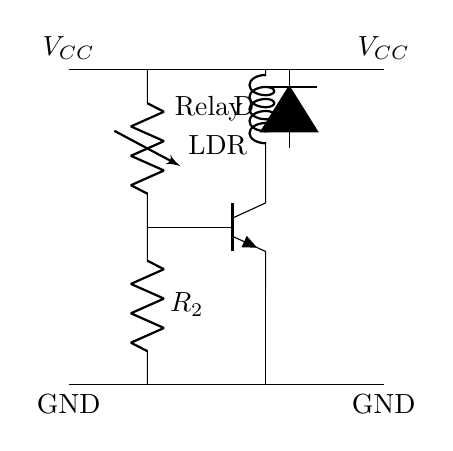
\begin{tikzpicture}[auto, node distance=2cm]
    \draw (0,4) node[above] {$V_{CC}$} -- (4,4) node[above] {$V_{CC}$};
    \draw (0,0) node[below] {GND} -- (4,0) node[below] {GND};
    
    % Divider
    \draw (1,4) to[vR, l=LDR] (1,2) to[R, l=$R_2$] (1,0);
    
    % Transistor
    \draw (2.5,2) node[npn](Q1){};
    \draw (1,2) -- (Q1.B);
    \draw (Q1.E) -- (2.5,0);
    
    % Relay
    \draw (Q1.C) -- (2.5,3) to[L, l=Relay] (2.5,4);
    \draw (2.8, 3) to[D*, l=D] (2.8, 4); % Flyback diode
    
\end{tikzpicture}
\captionof{figure}{Photo-Electric Relay Circuit}
\end{center}

\textbf{Working:}
\begin{enumerate}
    \item LDR resistance decreases when light falls on it
    \item Voltage divider (LDR + R2) provides base current to transistor
    \item Transistor turns ON when sufficient base current flows
    \item Relay activates when transistor conducts
\end{enumerate}

\begin{itemize}
    \item \keyword{Light Threshold}: Adjustable via potentiometer
    \item \keyword{Applications}: Automatic lighting, counting systems, alarm systems
    \item \keyword{LDR Characteristics}: Resistance inversely proportional to light intensity
\end{itemize}
\end{solutionbox}

\begin{mnemonicbox}
\mnemonic{Light Lowers Resistance, Transistor Turns, Relay Responds}
\end{mnemonicbox}

\questionmarks{4(c OR)}{7}{Draw the circuit of DC power control using SCR with UJT in triggering circuit and explain in detail.}

\begin{solutionbox}
UJT-triggered SCR circuit provides precise control of DC power to loads.

\begin{center}
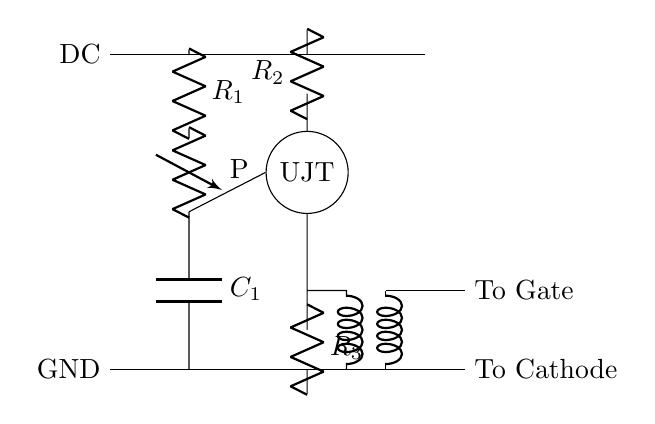
\begin{tikzpicture}[auto, node distance=2cm]
    % UJT Circuit
    \draw (0,4) node[left] {DC} -- (4,4);
    \draw (0,0) node[left] {GND} -- (4,0);
    
    \draw (1,4) to[R, l=$R_1$] (1,3) to[vR, l=P] (1,2) to[C, l=$C_1$] (1,0);
    \draw (2.5, 2.5) node[circle, draw] (UJT) {UJT};
    \draw (1,2) -- (UJT.west); % Emitter
    
    \draw (UJT.north) -- (2.5, 3.5) to[R, l=$R_2$] (2.5, 4);
    \draw (UJT.south) -- (2.5, 0.5) to[R, l=$R_3$] (2.5, 0);
    
    % Pulse Transformer
    \draw (2.5, 1) -- (3,1) to[L] (3,0); % Primary
    \draw (3.5,1) to[L] (3.5,0); % Secondary
    \draw (3.5,1) -- (4.5, 1) node[right] {To Gate};
    \draw (3.5,0) -- (4.5, 0) node[right] {To Cathode};
    
\end{tikzpicture}
\captionof{figure}{UJT Triggering Circuit}
\end{center}

\begin{center}
\captionof{table}{Circuit Components}
\begin{tabulary}{\linewidth}{|L|L|L|}
\hline
\textbf{Component} & \textbf{Function} & \textbf{Selection Criteria} \\ \hline
UJT & Generates trigger pulses & $\eta$ (intrinsic standoff ratio) = 0.5-0.8 \\ \hline
R$_1$+P & Timing resistor & Controls charging rate of C$_1$ \\ \hline
C$_1$ & Timing capacitor & Determines pulse frequency \\ \hline
Transformer & Isolates UJT circuit from SCR & Pulse transmission capability \\ \hline
SCR & Main power control & Current rating > load current \\ \hline
\end{tabulary}
\end{center}

\textbf{Working Principle:}
\begin{enumerate}
    \item UJT relaxation oscillator generates pulses
    \item Potentiometer varies charging rate, changing pulse frequency
    \item Pulses are coupled through transformer to SCR gate
    \item SCR conducts for portion of cycle based on trigger timing
\end{enumerate}

\begin{itemize}
    \item \keyword{Control Range}: From minimum to maximum power
    \item \keyword{Advantages}: Precise control, high efficiency
    \item \keyword{Applications}: DC motor control, heating elements, battery chargers
\end{itemize}
\end{solutionbox}

\begin{mnemonicbox}
\mnemonic{Resistor Regulates Rate, UJT Unleashes Pulses, SCR Switches Current}
\end{mnemonicbox}

% ==========================================================================================
% Question 5
% ==========================================================================================
\questionmarks{5(a)}{3}{Explain the hall effect sensor in BLDC driver circuit.}

\begin{solutionbox}
Hall effect sensors detect rotor position in BLDC motors for precise commutation timing.

\begin{center}
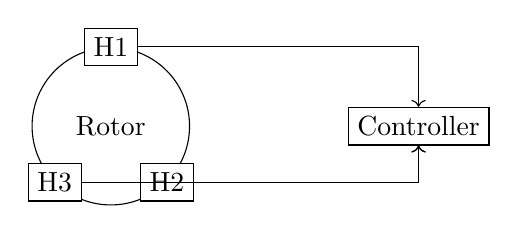
\begin{tikzpicture}[auto, node distance=2cm]
    \node [draw, circle, minimum size=2cm] (rotor) {Rotor};
    \node at (rotor.north) [draw, rectangle, fill=white] (H1) {H1};
    \node at (rotor.south east) [draw, rectangle, fill=white] (H2) {H2};
    \node at (rotor.south west) [draw, rectangle, fill=white] (H3) {H3};
    
    \node [draw, rectangle, right=2cm of rotor] (controller) {Controller};
    
    \draw [->] (H1) -| (controller);
    \draw [->] (H2) -| (controller);
    \draw [->] (H3) -| (controller);
\end{tikzpicture}
\captionof{figure}{Hall Sensor Placement}
\end{center}

\begin{center}
\captionof{table}{Hall Sensor Basics}
\begin{tabulary}{\linewidth}{|L|L|L|}
\hline
\textbf{Hall Sensor} & \textbf{Function} & \textbf{Output} \\ \hline
Position Detection & Senses magnetic field of rotor & Digital (ON/OFF) \\ \hline
Placement & 120\textdegree{} apart for 3-phase motors & Provides 6 unique states \\ \hline
Signal Processing & Inputs to microcontroller & Determines switching sequence \\ \hline
\end{tabulary}
\end{center}

\begin{itemize}
    \item \keyword{Working Principle}: Voltage generated perpendicular to current and magnetic field
    \item \keyword{Commutation Sequence}: Each sensor pattern corresponds to specific switching combination
\end{itemize}
\end{solutionbox}

\begin{mnemonicbox}
\mnemonic{Magnet Moves, Hall Senses, Controller Commutates}
\end{mnemonicbox}

\questionmarks{5(b)}{4}{Draw and explain solid state circuit to control speed of single phase Induction motor using TRIAC.}

\begin{solutionbox}
TRIAC-based speed control for induction motors uses phase control principles.

\begin{center}
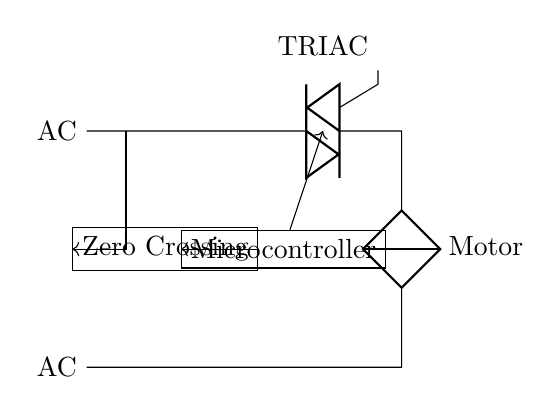
\begin{tikzpicture}[auto, node distance=1.5cm]
    \draw (0,3) node[left] {AC} -- (2,3) to[triac, l=TRIAC] (4,3) to[cisource, l=Motor] (4,0) -- (0,0) node[left] {AC};
    
    \node [draw, rectangle] (ZC) at (1, 1.5) {Zero Crossing};
    \node [draw, rectangle] (MC) at (2.5, 1.5) {Microcontroller};
    \draw [->] (0.5, 3) |- (ZC);
    \draw [->] (ZC) -- (MC);
    \draw [->] (MC) -- (3, 3); % Gate drive
    
\end{tikzpicture}
\captionof{figure}{Induction Motor Speed Control}
\end{center}

\textbf{Working Principle:}
\begin{enumerate}
    \item Zero-crossing detector identifies voltage zero-crossings
    \item Microcontroller calculates delay based on speed setting
    \item After delay, gate pulse sent through opto-isolator to TRIAC
    \item TRIAC conducts for remainder of half-cycle
    \item Varying firing angle controls voltage to motor, adjusting speed
\end{enumerate}

\begin{itemize}
    \item \keyword{TRIAC Rating}: Must handle starting current (5-7$\times$ running current)
    \item \keyword{Speed Range}: Limited at low end due to motor characteristics
    \item \keyword{Applications}: Fans, pumps, small machine tools
\end{itemize}
\end{solutionbox}

\begin{mnemonicbox}
\mnemonic{Zero Detected, Delay Determined, TRIAC Triggered}
\end{mnemonicbox}

\questionmarks{5(c)}{7}{Explain the construction and working of BLDC motor using diagram. Also enlist its applications.}

\begin{solutionbox}
Brushless DC motors use electronic commutation instead of mechanical brushes.

\begin{center}
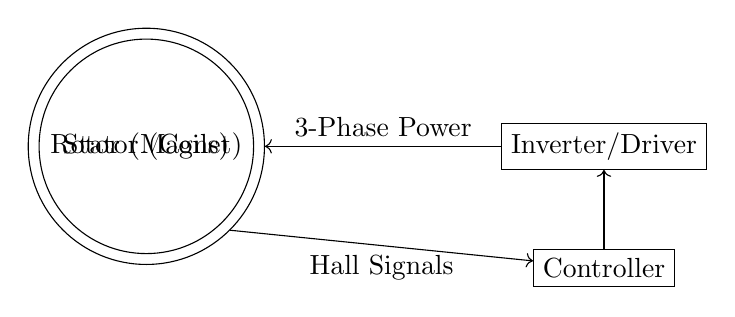
\begin{tikzpicture}[auto, node distance=2cm]
    \node [draw, circle, minimum size=3cm] (stator) {Stator (Coils)};
    \node [draw, circle, minimum size=1.5cm] (rotor) at (stator.center) {Rotor (Magnet)};
    
    \node [draw, rectangle, right=3cm of stator] (driver) {Inverter/Driver};
    \draw [->] (driver) -- (stator.east) node[midway, above] {3-Phase Power};
    
    \node [draw, rectangle, below=1cm of driver] (controller) {Controller};
    \draw [->] (controller) -- (driver);
    \draw [->] (stator.south east) -- (controller) node[midway, below] {Hall Signals};
    
\end{tikzpicture}
\captionof{figure}{BLDC Motor System}
\end{center}

\begin{center}
\captionof{table}{BLDC Components}
\begin{tabulary}{\linewidth}{|L|L|L|}
\hline
\textbf{Component} & \textbf{Function} & \textbf{Types/Variations} \\ \hline
Stator & Contains copper windings & Slotted/slotless designs \\ \hline
Rotor & Permanent magnets & Surface/interior mounted \\ \hline
Hall Sensors & Position detection & 60\textdegree{}/120\textdegree{} configurations \\ \hline
Controller & Commutation logic & Microcontroller-based \\ \hline
Driver & Power switching & MOSFET/IGBT-based \\ \hline
\end{tabulary}
\end{center}

\textbf{Working Principle:}
\begin{enumerate}
    \item Hall sensors detect rotor position
    \item Controller determines correct energizing sequence
    \item Driver powers appropriate stator windings
    \item Magnetic interaction produces rotation
    \item Process repeats continuously
\end{enumerate}

\textbf{Applications:}
\begin{itemize}
    \item Computer cooling fans and hard drives
    \item Electric vehicles and hybrid cars
    \item Industrial automation and robotics
    \item Medical equipment (pumps, ventilators)
    \item Drones and RC models
    \item Home appliances (washers, refrigerators)
    \item Precision instruments
\end{itemize}
\end{solutionbox}

\begin{mnemonicbox}
\mnemonic{Magnets Move, Sensors See, Electronics Energize}
\end{mnemonicbox}

\questionmarks{5(a OR)}{3}{Explain the working of variable frequency drive (VFD).}

\begin{solutionbox}
Variable Frequency Drives control motor speed by varying the frequency and voltage.

\begin{center}
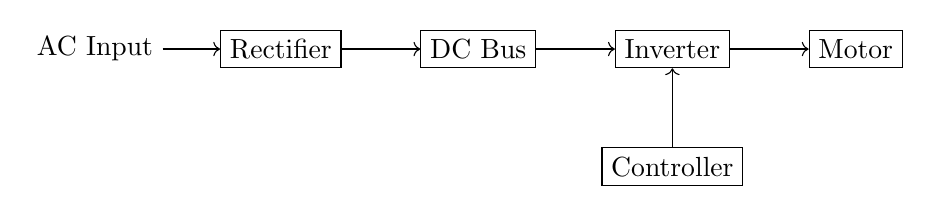
\begin{tikzpicture}[auto, node distance=2cm]
    \node [draw, rectangle] (rect) {Rectifier};
    \node [draw, rectangle, right=1cm of rect] (bus) {DC Bus};
    \node [draw, rectangle, right=1cm of bus] (inv) {Inverter};
    \node [draw, rectangle, right=1cm of inv] (motor) {Motor};
    
    \draw [->] (-1.5, 0) node[left] {AC Input} -- (rect);
    \draw [->] (rect) -- (bus);
    \draw [->] (bus) -- (inv);
    \draw [->] (inv) -- (motor);
    
    \node [draw, rectangle, below=1cm of inv] (control) {Controller};
    \draw [->] (control) -- (inv);
\end{tikzpicture}
\captionof{figure}{VFD Block Diagram}
\end{center}

\begin{center}
\captionof{table}{VFD Sections}
\begin{tabulary}{\linewidth}{|L|L|L|}
\hline
\textbf{VFD Section} & \textbf{Function} & \textbf{Components} \\ \hline
Rectifier & Converts AC to DC & Diodes or SCRs \\ \hline
DC Bus & Filters and stores energy & Capacitors, inductors \\ \hline
Inverter & Converts DC to variable AC & IGBTs or MOSFETs \\ \hline
Controller & Manages frequency/voltage & Microprocessor \\ \hline
\end{tabulary}
\end{center}

\begin{itemize}
    \item \keyword{V/f Control}: Maintains constant V/f ratio for stable torque
    \item \keyword{Operating Range}: Typically 10-200\% of rated speed
    \item \keyword{Efficiency}: High efficiency across wide speed range
\end{itemize}
\end{solutionbox}

\begin{mnemonicbox}
\mnemonic{Rectify to DC, Invert to AC, Vary Frequency}
\end{mnemonicbox}

\questionmarks{5(b OR)}{4}{Draw and explain the circuit to control speed of Universal motor.}

\begin{solutionbox}
Universal motors can run on AC or DC and allow simple speed control methods.

\begin{center}
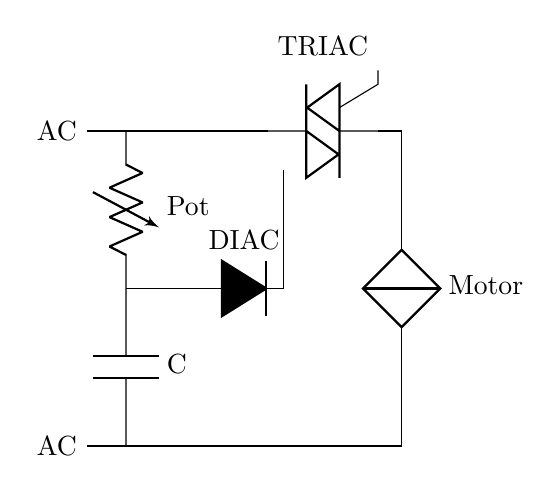
\begin{tikzpicture}[auto, node distance=1.5cm]
    \draw (0,4) node[left] {AC} -- (2,4) to[triac, l=TRIAC] (4,4) to[cisource, l=Motor] (4,0) -- (0,0) node[left] {AC};
    
    % Trigger
    \draw (0.5, 4) to[vR, l=Pot] (0.5, 2) to[C, l=C] (0.5, 0);
    \draw (0.5, 2) -- (1.5, 2) to[D*, l=DIAC] (2.5, 2) -- (2.5, 3.5); % To Gate
    
\end{tikzpicture}
\captionof{figure}{Universal Motor Speed Control}
\end{center}

\textbf{Working Principle:}
\begin{enumerate}
    \item RC network creates phase shift from input voltage
    \item Potentiometer adjusts phase shift amount
    \item DIAC triggers when voltage reaches breakover
    \item TRIAC conducts for remainder of half-cycle
    \item Adjusting potentiometer varies firing angle and motor speed
\end{enumerate}

\begin{itemize}
    \item \keyword{Speed Range}: Wide control range (10-100\%)
    \item \keyword{Torque Characteristics}: Decreases somewhat at lower speeds
    \item \keyword{Applications}: Power tools, household appliances, sewing machines
\end{itemize}
\end{solutionbox}

\begin{mnemonicbox}
\mnemonic{Resistance Changes Phase, DIAC Delivers, TRIAC Conducts}
\end{mnemonicbox}

\questionmarks{5(c OR)}{7}{Draw the block diagram of PLC and explain the function of each block in brief. And enlist the advantages and applications of it.}

\begin{solutionbox}
Programmable Logic Controllers (PLCs) are industrial computers for automation control.

\begin{center}
\begin{tikzpicture}[auto, node distance=2cm]
    \node [draw, rectangle, minimum height=2cm, minimum width=3cm] (CPU) at (0,0) {CPU};
    \node [draw, rectangle, minimum height=1cm, minimum width=2cm, left=1cm of CPU] (Input) {Input Module};
    \node [draw, rectangle, minimum height=1cm, minimum width=2cm, right=1cm of CPU] (Output) {Output Module};
    \node [draw, rectangle, minimum height=1cm, minimum width=3cm, above=1cm of CPU] (Power) {Power Supply};
    \node [draw, rectangle, minimum height=1cm, minimum width=3cm, below=1cm of CPU] (Mem) {Memory / Comms};
    
    \draw [->] (Power) -- (CPU);
    \draw [->] (Input) -- (CPU);
    \draw [->] (CPU) -- (Output);
    \draw [<->] (CPU) -- (Mem);
    
    \draw [<-] (Input.west) -- ++(-1,0) node[left] {Sensors};
    \draw [->] (Output.east) -- ++(1,0) node[right] {Actuators};
    
\end{tikzpicture}
\captionof{figure}{PLC Block Diagram}
\end{center}

\begin{center}
\captionof{table}{PLC Functions}
\begin{tabulary}{\linewidth}{|L|L|L|}
\hline
\textbf{PLC Block} & \textbf{Function} & \textbf{Types/Characteristics} \\ \hline
Power Supply & Provides regulated power & Typically 24VDC or 110/220VAC \\ \hline
CPU & Executes program, processes I/O & Scan-based operation \\ \hline
Input Modules & Interface with field sensors & Digital, analog, special \\ \hline
Output Modules & Control field devices & Relay, transistor, triac \\ \hline
Memory & Stores program and data & RAM, EEPROM, Flash \\ \hline
Communication & Network connectivity & Ethernet, Profibus, Modbus \\ \hline
\end{tabulary}
\end{center}

\textbf{Advantages:}
\begin{itemize}
    \item Reliability in harsh industrial environments
    \item Flexibility for reprogramming
    \item Compact size compared to relay-based systems
    \item Built-in diagnostics and troubleshooting
    \item Modular expandability
    \item High-speed operation
    \item Cost-effective for complex control systems
\end{itemize}

\textbf{Applications:}
\begin{itemize}
    \item Manufacturing production lines
    \item Process control in plants
    \item Material handling systems
    \item Building automation
    \item Power generation and distribution
    \item Water/wastewater treatment
    \item Packaging machinery
    \item Food processing
\end{itemize}
\end{solutionbox}

\begin{mnemonicbox}
\mnemonic{Power Provides, CPU Computes, Inputs Inform, Outputs Operate, Memory Maintains}
\end{mnemonicbox}


\end{document}
